%%
%% �����񍐗p�X�C�b�`
%% [techrep]
%%
%% �����p�X�C�b�`(keyword�͔C��)
%% [english]
%%

\documentclass[techreq,english]{ipsj}



\usepackage[dvips]{graphicx}
\usepackage{latexsym}
\usepackage{url}

\def\Underline{\setbox0\hbox\bgroup\let\\\endUnderline}
\def\endUnderline{\vphantom{y}\egroup\smash{\underline{\box0}}\\}
\def\|{\verb|}

\setcounter{volume}{22}% vol21=2013
\setcounter{number}{1}
\setcounter{page}{1}

%\received{2011}{7}{1}
%\rereceived{2011}{10}{1}   % optional
%\rerereceived{2011}{10}{31} % optional
%\accepted{2011}{11}{5}

\usepackage[varg]{txfonts}%%!!
\makeatletter%
\input{ot1txtt.fd}
\makeatother%

\begin{document}

\title{A Hybrid Game Contents Streaming Method to Improve Graphic Quality Delivered by Cloud Gaming}

\affiliate{NAIST}{Nara Institute of Science and Technology,Takayama-chou, Ikoma-shi, Nara 630-0192, Japan}
\affiliate{KU}{Kasetsart University, 50 Ngam Wong Wan Rd, Ladyaow Chatuchak, Bangkok 10900, Thailand}

\author{Kar-Long Chan}{NAIST}[kar\_long.chan.jr2@is.naist.jp]
\author{Kohei Ichikawa}{NAIST}[ichikawa@is.naist.jp]
\author{Putchong Uthayopas}{KU}
\author{Hajimu Iida}{NAIST}

\begin{abstract}
In gaming industry, Cloud Gaming is a new form of gaming service on trend trying to serve millions of players around the world with novel gaming experience. It aims to provide high-quality gaming service at any device, including thin clients which are incapable of handling high-definition gaming softwares. Players are only required to use any device that can connect to cloud servers for receiving streaming data through network and display game contents. Ideally Cloud Gaming is a promising service of providing novel gaming experience but in reality, various technological barriers make Cloud Gaming not comprehensively feasible for every type of game, such as first person shooting game which requires fast responsiveness. In addition, most existing cloud service, which streams encoded video sequence back to the client, is difficult to catch up with the rising demands for graphic quality. 
In this paper, the proposed hybrid game contents streaming method aims at improving graphic quality delivered from Cloud Gaming. Game contents streamed from cloud server are split into two parts, as one part is streamed as video sequence. Another part, which is streamed as graphic commands, is for rendering job to be performed at the client side. The locally rendered game contents are then displayed accordingly together with the contents streamed as video sequence. By taking the advantage of distributing rendering operation, the combined computing power is expected to produce better graphic quality. 
\end{abstract}

\begin{keyword}
Cloud Gaming, Hybrid-streaming method, QoE
\end{keyword}

\maketitle

%1
\section{Introduction}

Video Game industry has been considered as an essential sector in media industry, joining with the other two sectors including movie industry and music industry. The global market of video game is having rapid revenue growth, with an expectation of rising from 67 billion dollars in 2013 to 82 billion dollars\cite{gamingmarket} in 2017. In order to dynamically adjust to the complex and highly competitive business environment, video game industry is innovating its business model with the help of cloud technology. Efficiently utilising large amount of data through widely deployed data center helps to form the diversity of video game industry nowadays. Forms of video game business utilising cloud may include model of social usage, which can be recognised by many existing Massively Multiplayer Online Role-Playing Games (MMORPG) such as World of Warcraft and Finally Fantasy IX, together with games provided by social network based services. Another cloud-based video game business can refer to game contents delivery or distribution service, as Steam operated by Valve Corporation is among the most famous platforms in this segment of video game business. Cloud Gaming provides gaming services on demand, implying high accessibility to game contents from players. System of Cloud Gaming handles rendering, which is the most complicated part in contents processing, at the cloud servers and stream the encoded game scenes as video sequences to the player over network required with sufficient bandwidth, such as connection speed of 5 Mbits/s is recommended by OnLive\cite{Onlive} for smooth game play. At the player's side, control events from mice, keyboards, joysticks and other types of input devices are accurately recorded and transmitted from the player's machine back to the cloud servers for corresponding change of game logics. It is a relatively new business on trend having rapid development in term of technology and scale, and a forecast to reach 8 billion US dollars by 2017\cite{cggrowth} shows the evidence of tremendous market potential of Cloud Gaming.

The On demand nature of Cloud Gaming draws significant attention from both players and game developers for various reasons. As for the benefits of players, Cloud Gaming frees players from the complication of game software installation and management of compatibility with hardwares. With the mere requirement of thin client, which is a device being able to connect to network and display the received game scenes, players are granted with more different choices of platforms including PCs, laptops, tablets and smart phones to play games. In addition, players could pay less costs for more game choices. In term of advantages gained by game developers, Cloud Gaming eases the possible imcompatibility issues between hardwares and softwares. Therefore, developers are easier to adapt their game softwares to more different platforms, thus decreasing the production costs and increasing the net revues. Features of Cloud Gaming envision a promising future of providing million players with novel gaming experience, as it has been an active topics both in industries and research fields recently. OnLive is a leading Cloud Gaming service providers based in San Francisco USA providing game software from over 50 publishers. Sony's acquisition of Cloud Gaming company Gaikai\cite{Gaikai} in the year of 2012 shows great interests toward Cloud Gaming from leading media enterprises. GamingAnyWhere\cite{huang2013gaminganywhere}, developed by Shen-Wei Chen, is an open-source Cloud Gaming platform available for the use of research. 

However, maintaining and improving quality of experience (QoE) is considered to be very challenging in Cloud Gaming services because networking constraints become majorly significant. Design of Cloud Gaming system must be able to dynamically adapt to varied network conditions in order to preserve stable quality. Previous research have perform excessive performance evaluation\cite{chen2011measuring, huang2013gaminganywhere} for multiple existing Cloud Gaming platforms including OnLive, StreamMyGames\cite{SMG} and GamingAnyWhere, based on Frame Rate and Video Quality metrics including PSNR and SSIM. Network emulation tool such as dummynet\cite{rizzo1997dummynet} has been applied for injecting delay, packet loss and bandwidth to simulate different network conditions. Results of evaluations show that Frame Rate Per-second in most platforms degrade in unstable network environment such as long network delay, high packet loss and limited bandwidth.  In addition, similar degrades can be found in Video Quality, as it is also vulnerable to bad network connection. Among the tested platforms, Cloud Gaming service provider OnLive maintains relatively stable performance.

Another subjective test being conducted has found that players are sensitive to changes in graphic quality and smoothness during game plays\cite{jarschel2011evaluation}. This implies that video quality plays an important role in Cloud Gaming experience, especially for those games which rely on impressive visuals. Nowadays many game softwares, particularly for those major contenders, largely depend on realistic visual effects to keep up with their competitiveness in the market. However, games chosen for previous evaluations are considered to be conservative in term of visual effects compared to other available titles. In addition, lack of new titles served by Cloud Gaming provider such as OnLive shows the lack of confidence to run the newest game softwares  on present Cloud Gaming platform. Furthermore, game content streamed at resolution of 720p (1280 x 720) is fixed  for every game in OnLive in order to maintain fairness in delivering service. Compared with game contents served as the standard of Full HD (1920 x 1080) to even 4K (3840 x 2160) quality in most traditional gaming platforms, including game consoles and PCs, quality of 720p appears to be marginal. However, since most effort has been spent on maintaining QoS by balancing video quality and response delay, there is no significant study on improving graphic quality provided by Cloud Gaming. Therefore, it is necessary to look for approach to improve delivered graphic quality in order to keep up the competitiveness of Cloud Gaming.

In this paper, a hybrid game contents streaming method is proposed aiming at improving graphic quality delivered from Cloud Gaming. The concept of hybrid streaming here refers to the method  constructed from both video-based streaming and instruction-based streaming, as these two terms will be explained in later section. By using the proposed method, game contents streamed from cloud server are split into two parts, as one part is streamed as video sequence. Another part, which is streamed as graphic commands, is for rendering job to be performed at the client side. The rendered game contents are then displayed accordingly with the contents streamed as video sequence. By taking the advantage of distributing rendering operation, the combined computing power is expected to produce better graphic quality.

At the present stage of work, a very basic prototype has been constructed based on the only available open-source Cloud Gaming platform, GamingAnyWhere. In addition, a custom OpenGL demo has been used for evaluating the graphic quality using the metric of PSNR.
Eisert 
The remainder of the paper is structured as follows. In Section II two important terms related Cloud Gaming are explained and some existing Cloud Gaming platforms and their technologies will be briefly introduced. Section III explains the proposed method in details and the status of present works together with the evaluation. In Section IV, we discuss about the validation to the concept of the proposed method. Finally, in Section V, we give a conclusion and provide an outlook on future work.

\begin{figure*}[t]
\centering
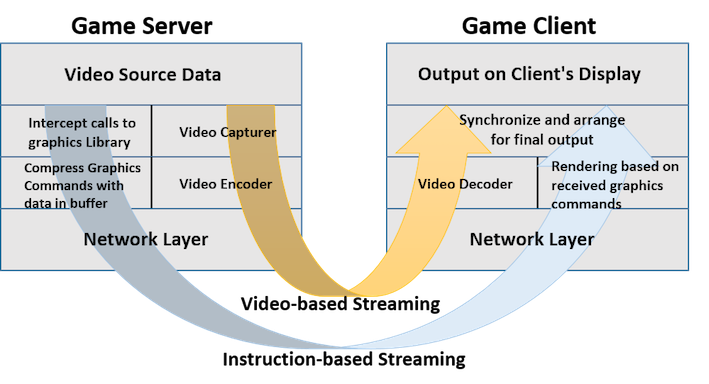
\includegraphics[scale=1]{hybridmodel.png}
\caption{An overview of our proposed hybrid-streaming model}
\label{fig:hybrid}
\end{figure*}

%2
\section{Related Works}
Cloud Gaming system can be regarded as a type of real-time remote rendering system, as the technology in behind is similar to remote application such as Remote Desktop. However, dedicated video player and encoder are usually specifically designed for the use of Cloud Gaming, which guarantee an environment to handle more rigid real-time response. In general, the streaming approaches of Cloud Gaming system can be categorised into two types, video streaming and instruction streaming. These two methods differ from each other in how the game contents are divided between the server and the client.
%2.1
\subsection{Video-based Streaming}
In the system with video streaming approach, game logics are calculated at the server CPU and the 3D graphics renderings are processed through the dedicated Graphic Processing Unit at the server. The rendered contents are then compressed into 2D video and streamed to the client. At the client side, the received streaming of video is decoded and the corresponding game contents are shown on the client's display. Since the decoding can be done by using low-cost decoder chips which are massively embedded in consumer's electronics, this approach is ideal for thin client running on source-constrained devices. In addition, this approach also suits well with the concept of Cloud Gaming, by freeing client from complicated 3D operations. Therefore, most of the existing commercial Cloud Gaming platforms such as OnLive, StreamMyGame are using this approach in their systems. OnLive is one of the leading Cloud Gaming service providers in the market, as it is famous for providing fair and stable streaming of game contents by using dedicated servers and highly specialised encoding hardwares and algorithms. All games provided by OnLive are streamed at the quality of 720p. StreamMyGame is a game streaming solution that allows players to setup their own Cloud Gaming environment, which allows players to stream their own games through network. Furthermore, GamingAnyWhere is the first and the only available open source Cloud Gaming platforms. There are two video capture modes in GamingAnyWhere, the hooking mode and desktop streaming mode, which will be explained more specifically in later section. According to evaluation done in previous research, GamingAnyWhere outperforms the other two Cloud Gaming platforms including OnLive and StreamMyGame in term of response and graphic quality under a good network environment. However, it is not as stable as OnLive if the environment becomes varied.

%2.2
\subsection{Instruction-based Streaming}
As for the instruction streaming approach, the graphics commands are intercepted and compressed at the server side, and then streamed to the clients. The clients then render the game contents using its local graphic processing units based on the received graphics commands. Eisert at el\cite{eisert2008low} implements this approach in the framework of Game@Large\cite{nave2008games} by intercepting calls to the OpenGL library as well as the SDL library at the server. Then, the graphics commands set is efficiently compressed with corresponding objects and textures and streamed to the client for local rendering. Therefore, this approach requires graphic processing unit at the client side not only compatible with the streamed graphics commands such as OpenGL and Direct3D, but also powerful enough to render the game contents in real time and high quality. Since graphics unit at the server side is not used in this approach, multiple games can be executed in one server simultaneously and it is suitable for providing services within small scale network community. However, imposing more workload on clients makes this approach not a viable option for source-constrained devices.

%2.3
\subsection{Other approaches}
Beside these two major streaming methods, an approach of video streaming with post-rendering operation is also proposed\cite{shi2011using}. This method is majorly designed for cloud-based mobile game usage. Compared to broadband network, wifi connection of mobile device implies much smaller bandwidth and possible longer latency. Therefore, this approach aims to enhance video encoding for cloud-based mobile gaming service by taking the advantage of run-time graphics rendering contexts form 3D game engine. In this method, the modified encoder selects a set of key frames in the video sequence, uses a 3D warping algorithm based on the context data from the game engine to interpolate other non-key frames. The interpolation allows encoding warping residues with much lower bit rate, while maintaining or even improving video quality. 

%3
\section{Hybrid Streaming approach}
In this paper, we propose a hybrid streaming approach (\figref{fig:hybrid}) which splits the game contents data into instruction-based streaming and video-based streaming, aiming to achieve better video quality at the client's side by combining products from these two streams. The idea of this approach is from Scalable Link Interface (SLI), a multi-GPU technology developed by NVIDIA for linking two or more Graphic Cards together to increase the processing power available for a single graphic output. Certainly the transfer rate in the network environment of Cloud Gaming cannot match with the local PCI-E speed of graphic Card, but the concept of distributing 3D processing workload into different  graphics processing units can be taken as reference to manipulate data in Cloud Gaming system. 

%3.1
\subsection{Process of Video-based Streaming}
Our hybrid approach is implemented upon the existing open source Cloud Gaming platform GamingAnyWhere, which uses video-based streaming approach to deliver game contents. The well implemented mechanism of handling video source achieves impressive result in previous evaluations, which gives us confidence that no significant modification for video streaming is needed in our system. In the structure of GamingAnyWhere, two types of network flows are defined, the data flow and the control flow. Data flow is used to stream audio and video frames from the server to the client while in a reverse direction, control flow is used to send user's actions including inputs from keyboard, mice from the client to the server. In this paper, we will focus on the mechanism of video source handling at the server. Two video source capture modes are implemented in GamingAnyWhere,  Desktop Capture mode and API Intercept mode. Desktop Capture mode captures the entire desktop screen at a specified rate while the API Intercept mode hooks drawing APIs from the game and captures the screen directly from the game's back buffer. The captured raw data is then sent to the encoder for encoding. Finally the encoded data is delivered through network connection based on either TCP or UDP protocol, which can be specified based on the preference of the user. In our system, part of the game contents data, which is represented as objects, vertex arrays or textures,  undergoes this stream of process: Rendered as 2D image through server's graphic card and encoded as video sequence, and then streamed to the client. At the client side, the video sequence is decoded and shown on player's display. Since the workload of rendering task at the server side is lightened, we can expect an increase of efficiency at the same time. In addition, libavcode library, which is part of ffmpeg project\cite{bellard2006ffmpeg}, is used as the encoding module in GamingAnyWhere and because of the high extensibility of this library, we can use any codec supported by libavcodec. 

%3.2
\subsection{Process of Instruction-based Streaming}
As for another part of game contents data, it is streamed as graphics commands to the client and rendered by using client's graphics cards. Similar to previous approach, the proposed system will intercept all calls to graphics rendering libraries such as OpenGL, Direct X as well as SDL. Regarding other corresponding data such as vertices and textures being stored in buffers, we are currently considering two approaches to handle such data. One is based on Eisert's proposal, by efficiently compressing all these data with the graphics commands set for streaming. Another approach is to have a copy of texture and objects data at the client side from the beginning, so only the graphics commands set is streamed to the client. Then at the client side, the rendering operation can be performed by loading corresponding datas from the client's device. Since only graphics commands set is delivered to the client, transferring with low bit rate can be guaranteed. For the second approach, we also need to setup an assumption for the usage of the proposed system, which will be stated in later section.

%3.3
\subsection{Final product of the game contents}
How the final representation of game contents is correspondingly formed from the products of two different streams is another important design objective, which should largely depend on how the game contents data is split at the server. At present, we are considering to compare the depth value of each object in one frame. Based on the depth value, all the objects are separated into two groups, the upper layer which contains shallower objects and the lower layer which contains deeper objects. Considering that the contents delivered through video-based streaming result in video frame without z value, the game contents shown in this form should be used as background. For this purpose, objects belonging to lower layer are streamed as video sequence. On the other hands, objects belonging to upper layer are streamed as graphic command sets. Therefore, as soon as the rendering operation is completed at the client side, the resulted contents can be pasted on the background represented by the contents streamed as video sequence. Furthermore, each video streaming packet delivered from GamingAnyWhere server comes with a marker bit, which is for indicating  that the current packet belongs to the same frame. By applying the same mechanism of embedding a marker bit into each packet carrying the graphics commands in instruction-based streaming, contents rendered at the client side should  synchronise accordingly with the contents from video-based streaming.

%4
\section{Implementation and Evaluation}
In order to construct the proposed hybrid streaming model, we implemented the system based on the platform of GamingAnyWhere. As the first step in our implementation, we created a very simple prototype to evaluate the video quality. Instead of manipulating all the data at the server, the current implementation directly loads an OpenGL object, which is pre-installed at the client side ,and pastes the rendered result on the other contents streamed as video sequence from the server side. Afterwards, we conducted the evaluation by using the metric of PSNR.
%4.1
\subsection{Environment setup}
We installed the GamingAnywhere pre-compiled package, which comes with both client module and server module, on two machines, as one is for server and another one is for client . The server machine is equipped with an Intel Core i7 4770K 3.5GHz CPU, a Nvidia GeForce GTX 780 graphic card and 16GB system memory, running as a 64-bit Linux system. As for the client machine, it is a Mac Book Pro equipped with a 2.6 GHz Intel Core i7 CPU, a Nvidia GeForce GT 750M with 16GB system memory. After successfully installing GamingAnyWhere, we had our system operate in the campus network environment, which is considered to be sufficient in our implementation. 

In order to stream a game in GamingAnyWhere, the platform provides an easy way of executing either in Desktop Capture mode or API Intercept Mode (Hooking Mode) by inputting a simple command line in CLI. The command takes a configuration file as parameter, in which we specify the window we want to capture if using the Desktop Capture mode. Otherwise, we specify the gaming software execution file we want to intercept if using the Hooking Mode. Many other parameters such as encoding bits, rate of capturing and pixel formats can be set within the configuration file.

For achieving the best graphic quality, the hooking mode is ideally the best option since it takes more original raw data directly from the back buffer. However, the hooking-mode is not supported in a 64-bit Linux system and hence, the desktop capturing mode is the only option in current implementation. The encoder is H.264, which is the default configuration come with GamingAnyWhere, and the data is streamed as H.264/MPEG-4 AVC format. 

\begin{figure}[t]
\centering
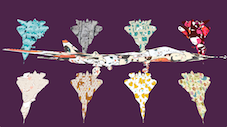
\includegraphics[scale=1]{original.png}
\caption{Screenshot of demo application}
\label{fig:demo}
\end{figure}

%4.2
\subsection{Demo application for current evaluation}
At current stage of the implementation, taking the use of existing game software as test case is difficult because the data in the software can be large and complicated. Instead, we decided to create our own simple demo application for the current evaluation by using graphics commands library OpenGL. Before creating this demo application, we established two design objectives to base on. First, this application should have distinguished front objects and background objects, which allows us to easily split the contents into video-streaming and local rendering. Secondly, since the mechanism of synchronisation has not been implemented yet, the outcome of the application should not be largely affected by the necessity of synchronisation, which helps to perform more valid evaluation as well. 

Based on these two design objectives, we created a demo application which is shown in \figref{fig:demo}.  In this demo, there are 8 jet-fighter models spinning counter-clockwise along the x-axis. In the foreground, there is a bigger jet-fighter model statically showing on the screen. With this application, we could easily separate the 8 spinning jet-fighter models for video streaming from the server, and the bigger static model for being rendered at the client side. Furthermore, since the foreground object is static, the influence of synchronisation is considered to be not significant, which allows us to confidently capture frame from the demo and perform comparison with reference model in the evaluation.
%4.3
\subsection{Source Code Modification}
Since the instruction-based streaming has not been implemented yet in the current prototype, there is no modification done at the server side, in which the video-based streaming is the only streaming mechanism. In our prototype implementation, most of the source code modification was done at the client module. The original module implementation of GamingAnyWhere client takes the incoming streaming data, which is represented as a ffmpeg data structure called AVPicture, and converts it to SDL\_Texture. By using SDL API functions SDL\_RenderCopy and SDL\_RenderPresent, the contents which are now stored as SDL\_Texture are shown on the display by using SDL type renderer. 

In our modification, which is represented in \figref{fig:workflow}, we created a Mesh class based on OpenGL library that can load the object file of the jet-fighter. This object file, which ends with .obj, is created by using Blender, a professional OSS for 3D computer graphics. Generally, this object file stores all the vertices to construct the object, which is the jet-fighter in our current implementation. By loading the object file into the VertexArray of OpenGL, client's graphic card render the object based on a pre-specified OpenGL context. After SDL\_RenderPresent has shown the contents from video-streaming, we swapped the SDL rendering context into OpenGL context by using SDL\_GL\_MakeCurrent. Finally, we used SDL\_GL\_SwapWindow to display the rendered jet-fighter upon the contents from video streaming.


\subsection{Result and Evaluation}
The implemented prototype successfully overlays the static jet-fighter object upon the contents streamed from the server. However, possibly due to the reason that SDL based renderer is not well compatible with OpenGL based renderer, the texture is not bound appropriately on the object. A solution for this problem is considered and it will be discussed in next section.

\begin{figure}[t]
\centering
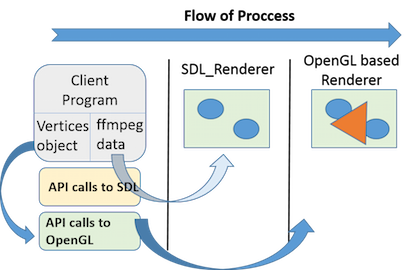
\includegraphics[scale=1]{current_implmentaion.png}
\caption{Work flow of current implementationl}
\label{fig:workflow}
\end{figure}


As for the preliminary evaluation of graphic quality, we applied the metric Peak Signal-To-Noise ratio (PSNR) to compare between our hybrid model and video streaming. In order to take the measurement of PSNR, we used a window capture software Screenflick to capture a short video at 60fps for the demo application running in video-streaming mode, hybrid mode and at original quality which is the reference source that PSNR measurement needs to base on. The setting of this window capturing is configured to be as high quality as possible for the purpose of retaining the original quality. After acquiring a video source for each mode, we used a command of ffmpeg to extract every frame from the video source. Then from each video source, we picked a frame with the most similar background motion to one another, due to the fact that the jet-fighter in foreground is static. Finally, we used a compare command from ImageMagicK to retrieved the PSNR metric from both hybrid model and video streaming based on the chosen frames. 

As shown in \tabref{tab:PSNR}, the PSNR result achieved from video-based streaming is 28.36 compared to 20.06 from hybrid model, which implies that the video quality from video streaming is better than the current hybrid implementation. This can be understandable as being mentioned in previous paragraph, the texture in hybrid model does not bind on the object appropriately, which causes significant difference from the reference frame. For temporarily addressing this issue, we conducted another evaluation by applying monotone texture, which binds accordingly on the jet-fighter object. As for the result (shown in \tabref{tab:PSNR_better}), our hybrid implementation and video streaming achieve 28.80 and 26.11 respectively, implying better outcome of our model compared to video-streaming approach and previous evaluation.

\begin{table}[t]
\caption{Result of PSNR from video-based streaming and current hybrid model}
\label{tab:PSNR}
\centering
\begin{tabular}{lrr}
\hline
&Video-Streaming&Current Hybrid Model\\\hline
PSNR&28.36&20.06\\\hline
\end{tabular}
\end{table}

\begin{table}[t]
\caption{Result of PSNR from video-based streaming and current hybrid model, using monotone texture}
\label{tab:PSNR_better}
\centering
\begin{tabular}{lrr}
\hline
&Video-Streaming&Current Hybrid Model\\\hline
PSNR&26.11&28.80\\\hline
\end{tabular}
\end{table}


%5
\section{Discussion}
In this session, we address the issue that we discovered in our implementation, and also we state our expectation of this hybrid system's position in term of market value and user's benefit.

%5.1
\subsection{Considered solution for incompatibility}
As mentioned in previous section, the uncoordinated binding of texture on the jet-fighter model is considered to be the outcome of incompatibility between SDL based renderer and OpenGL based renderer. In normal use case, SDL library cooperates well with OpenGL if SDL is mainly used for managing input mechanisms and sound while leaving the rendering tasks, especially 3D processing, to OpenGL. However, in our current system, both SDL based renderer and OpenGL rendering context are utilised at the same time, which is likely to cause conflicts at buffer level and result in an unexpected behaviour of texture binding. In order to solve this problem, we plan to convert ffmpeg data structure AVPicture directly into OpenGL Texture data, by which we use OpenGL rendering context as the only renderer in our implementation without worrying about the stated conflicts.
%5.2
\subsection{Position of Our System}
Highly accessible to game contents is the core idea of Cloud Gaming, as most existing service providers emphasise on the point that high quality games can be available for playing on any device. It frees users from the complication of installing the gaming softwares and upgrading their systems for newer games. However, standing from the position of potential users of Cloud Gaming, the devices that they own may actually equip with graphic processing unit such as graphic cards, especially for many PC game players. To this group of potential users, Cloud Gaming is attractive in the way of highly accessible to game contents, but not the graphic quality which is represented as encoded video stream. Compared to having a copy of game software run at local side for smoother gameplay with better graphic quality, the advantage of Cloud Gaming becomes marginal. Therefore, increasing the value of Cloud Gaming from user's perspective becomes our motivation to develop this hybrid streaming model. By effectively utilising resources from both server side and client side, we expect the system is eventually able to offer graphic quality that matches with local rendering. 

%6
\section{Conclusion}
In this paper, we present our idea of implementing a hybrid streaming method to enhance the graphic quality offered by Cloud Gaming. This method is based on video-streaming and instruction-streaming, which are the two major approaches used in existing Cloud Gaming platforms. Our goal is to use this hybrid streaming to utilise graphics processing power on both client side and server side to eventually achieve better graphic quality, that possibly matches with local rendering. We expect that this hybrid-streaming method can help to increase the value of Cloud Gaming service from user's perspective. 

We also implemented a simple prototype based on GamingAnyWhere for preliminary evaluation of the method. The result shows that the graphic quality, which is measured as PSNR, from video-streaming is better than the one from the current implementation, as the reason is considered to be the imcompatibility between SDL and OpenGL.

As for the future work, we will fix the imcompatibility issue by using only OpenGL renderer. Afterwards, we will develop a better demo application for evaluation and then move on to the implementation of whole system, starting from the mechanism of instruction streaming at the server side. 


\bibliographystyle{ipsjunsrt-e}
\bibliography{bib_db}

\end{document}
